\section{CAD第四次作业}
\setcounter{subsection}{0}
\subsection{题目:}

\tt{通过仿真，确认如图的输入电阻，输出电阻，等效诺顿流与电压放大倍数的分析正确}

\begin{figure}[H]
\centering
\resizebox{0.7\textwidth}{!}{%
\begin{circuitikz}
\tikzstyle{every node}=[font=\large]
\draw (2.5,11) to[american voltage source] (2.5,8.25);
\draw (2.5,13.75) to[european resistor,l={ \small $R_{s}$}] (2.5,11);
\draw (4,13.75) to[european resistor,l={ \small $r_{be}$}] (4,11);
\draw (8,13.75) to[european resistor,l={ \small $r_{ce}$}] (8,11);
\draw (5,10.75) to[european resistor,l={ \small $R_{e}$}] (5,8.25);
\draw (2.5,8.25) to[short] (8.75,8.25);
\draw (8.75,13.75) to[european resistor,l={ \large $R_{L}$}] (8.75,8.25);
\draw (2.5,11) to[short] (8,11);
\draw (5,11) to[short] (5,10.5);
\draw (2.5,13.75) to[short] (4,13.75);
\draw (7.5,13.75) to[short] (8.75,13.75);
\draw (6.25,13.75) to[short] (7.5,13.75);
\draw (6.25,13.75) to[american controlled current source,l={ \small $g_{m}V_{be}$}] (6.25,11);
\node [font=\large] at (4,14.25) {b};
\node [font=\large] at (6,10.75) {$e$};
\node [font=\large] at (6.5,14.25) {$c$};
\end{circuitikz}
}%

\label{fig:my_label}
\end{figure}
\tt{其中$R_{s}=100\Omega$，$R_{e}=1k\Omega$，$R_{L}=10k\Omega$，$r_{be}=1k\Omega$，$r_{ce}=100k\Omega$，$g_{m}=40mS$}

\subsection{理论计算:}

\tt{输入电阻：$R_{in}=r_{be}+R_{E}\frac{r_{ce}+R_{L}+g_{m}r_{be}r_{ce}}{r_{ce}+R_{L}+R_{E}} =371.4k\Omega $}

\tt{输出电阻：$R_{out}=r_{ce}+R_{E}\frac{r_{be}+R_{S}+g_{m}r_{be}r_{ce}}{r_{be}+R_{S}+R_{E}} =3.705M\Omega $}

\tt{等效诺顿电流源：$I_N=V_S\frac{R_E-g_mr_{be}r_{ce}}{r_{ce}(r_{be}+R_S)+R_E(r_{be}+r_{ce}+R_S+g_mr_{be}r_{ce})}=-972.7V_S$}
\tt{其中-972.7的量纲为uS}

\tt{电压放大倍数：$V_L=I_N\frac{R_NR_L}{R_N+R_L}=-9.701V_S$}
\tt{,即19.7dB反相}

\subsection{输入电阻：}

\begin{figure}[H]
\centering
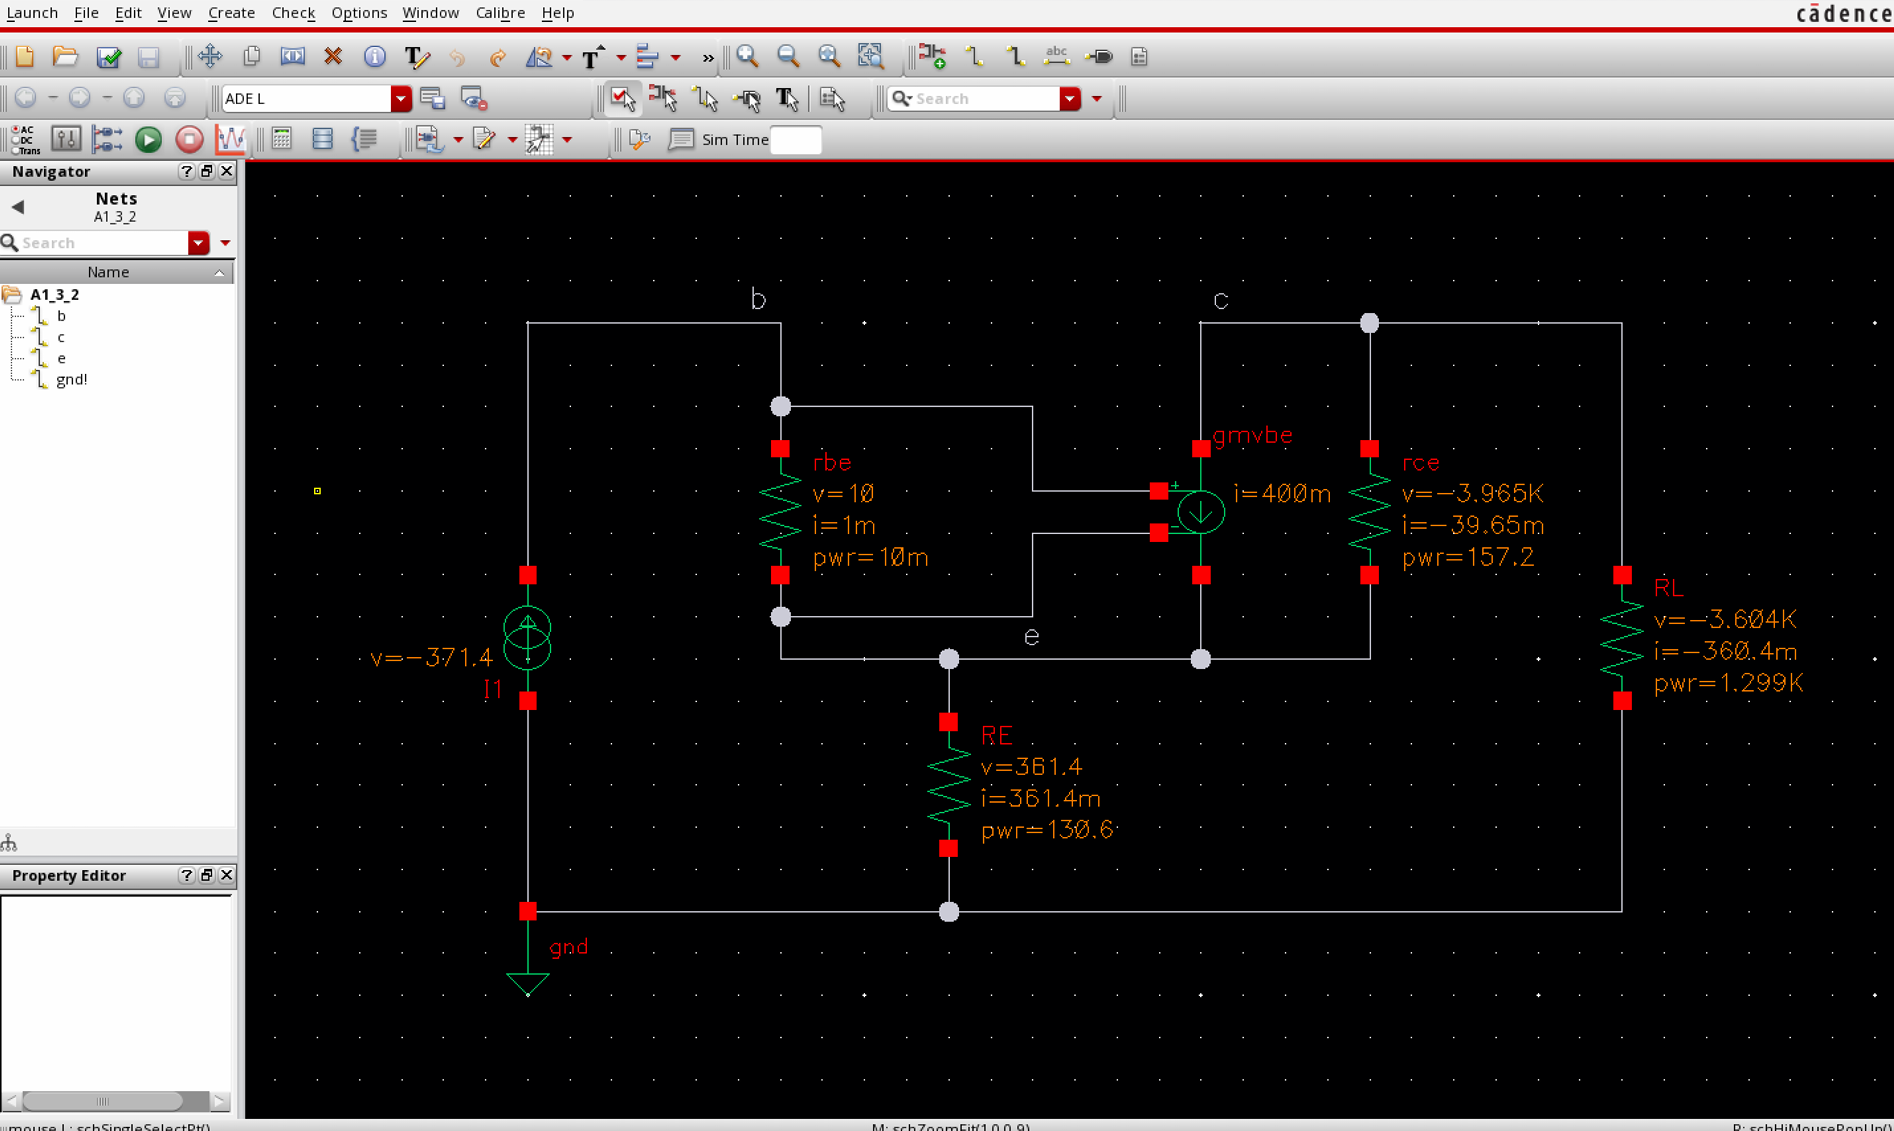
\includegraphics[width=1\textwidth]{chapters/figure/A4/A4input.png}
\caption{输入电阻仿真结果}
\label{输入电阻仿真结果}
\end{figure}

\tt{给恒流源加1mA电流，仿真得到输入电阻为$R_{in}=371.4k\Omega$，与理论计算结果一致}

\subsection{输出电阻：}

\begin{figure}[H]
\centering
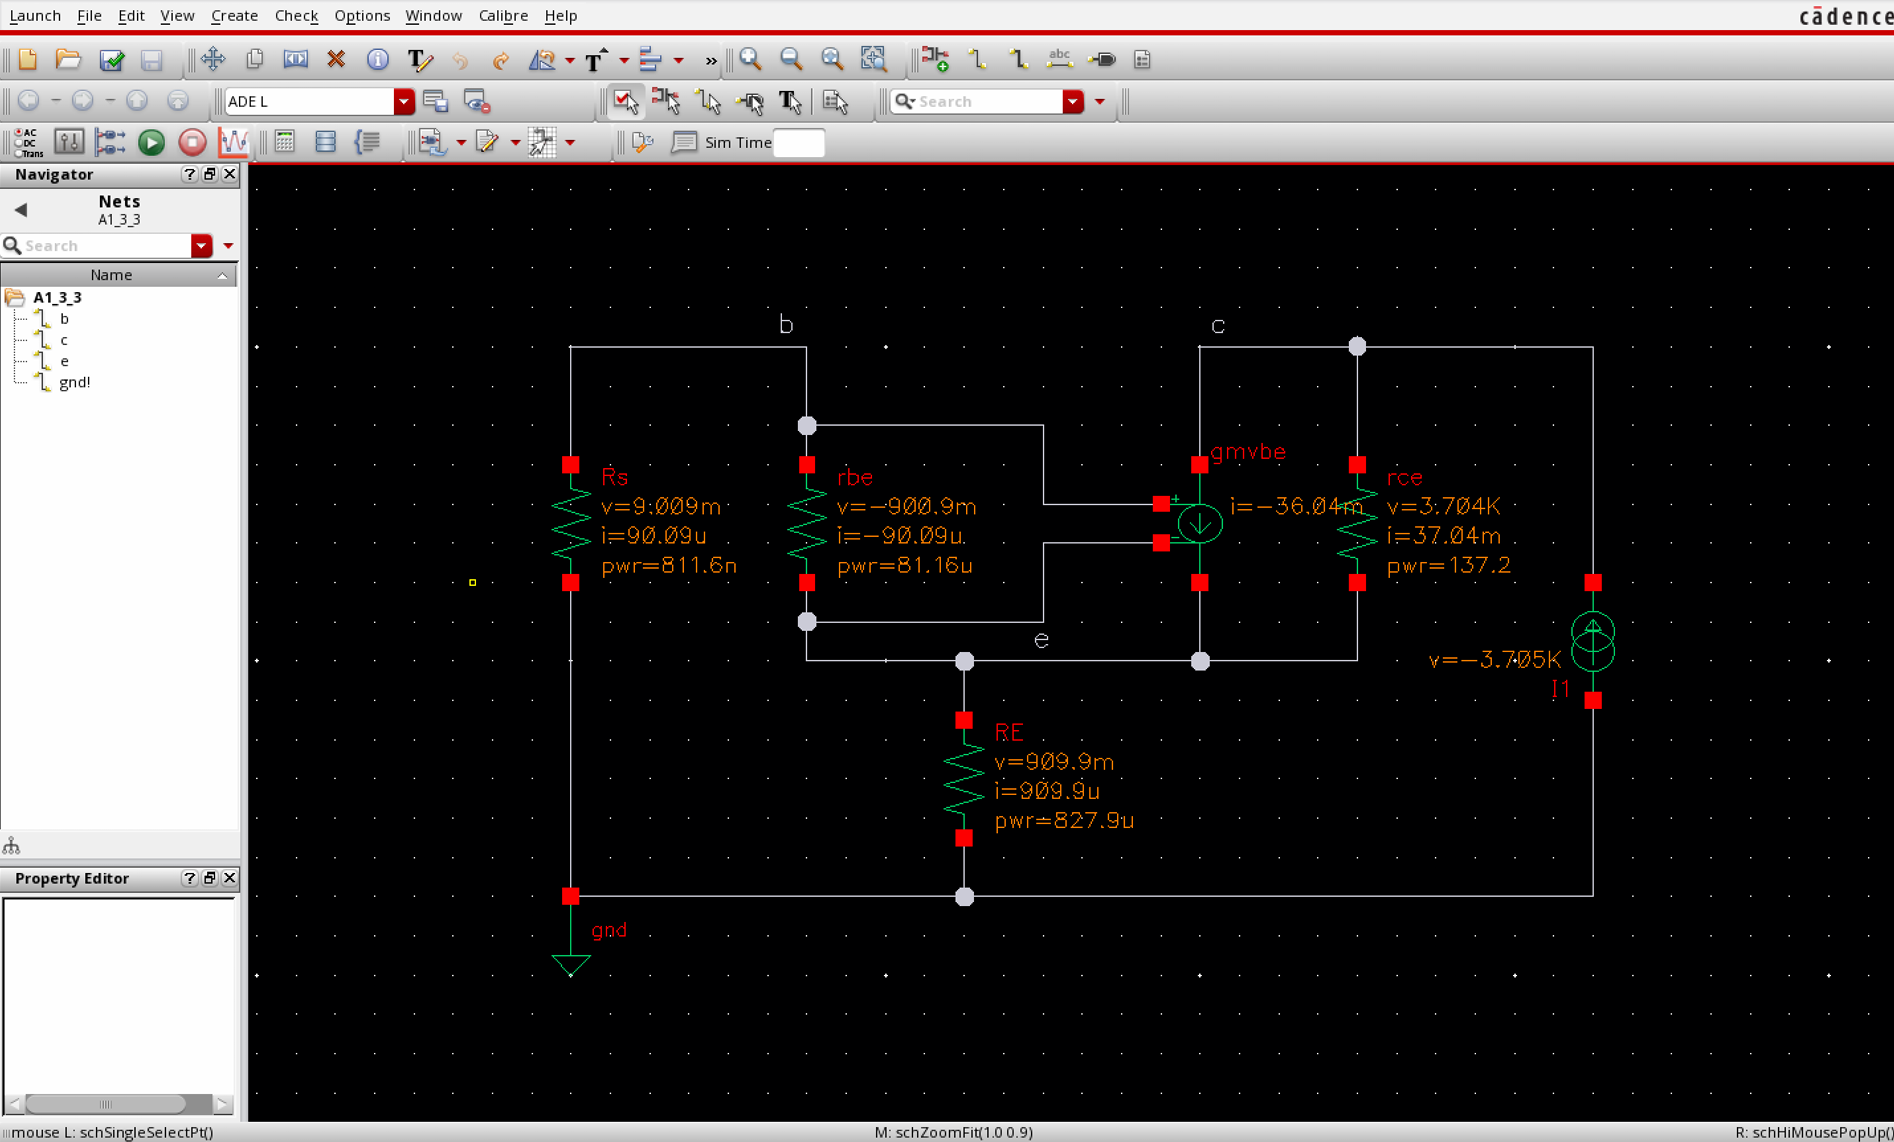
\includegraphics[width=1\textwidth]{chapters/figure/A4/A4output.png}
\caption{输出电阻仿真结果}
\label{输出电阻仿真结果}
\end{figure}

\tt{给恒流源加1mA电流，仿真得到输出电阻为$R_{out}=3.705M\Omega$，与理论计算结果一致}

\subsection{电压放大倍数：}

\begin{figure}[H]
\centering
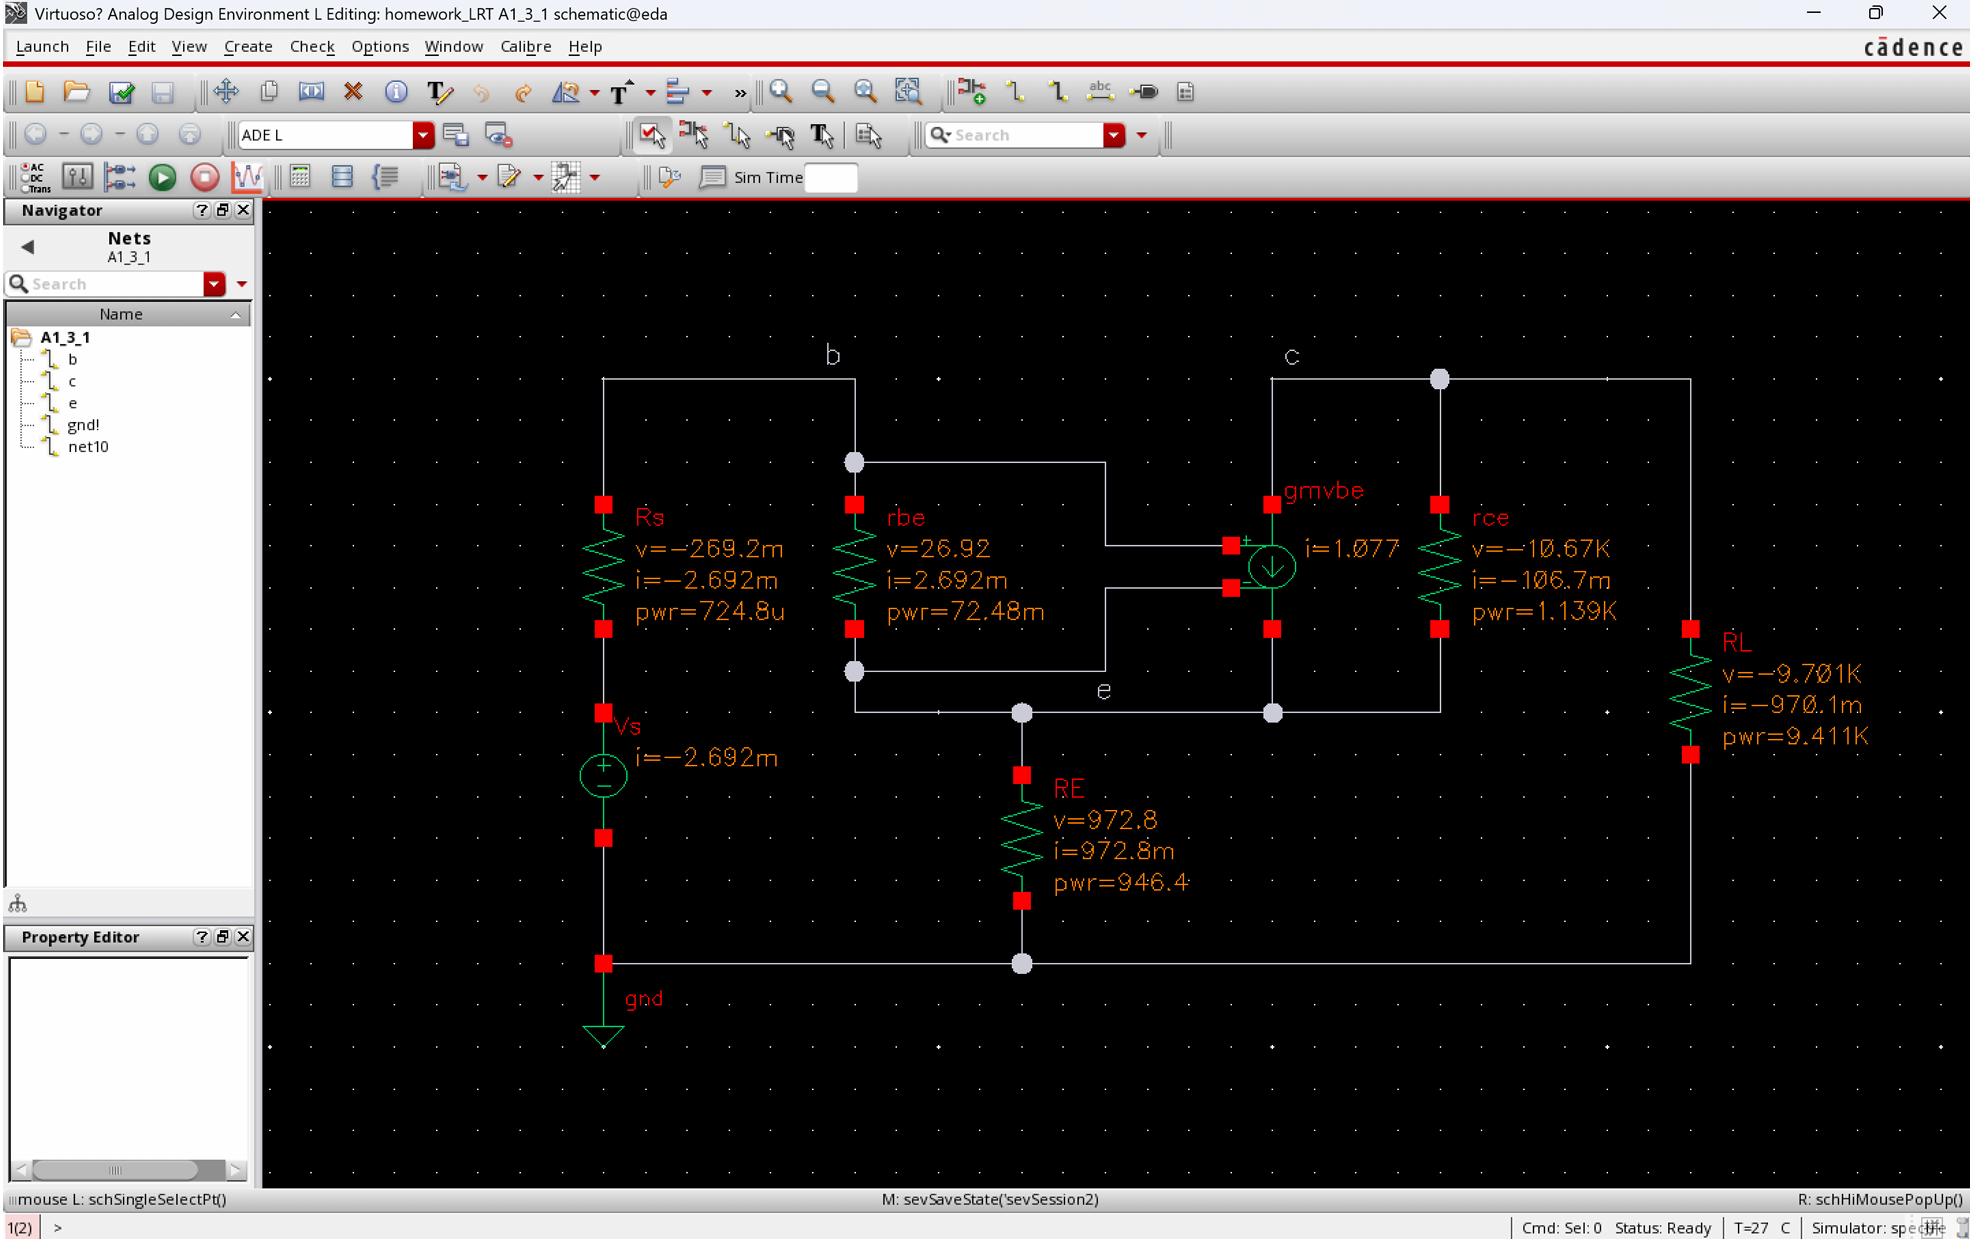
\includegraphics[width=1\textwidth]{chapters/figure/A4/A4AV.png}
\caption{电压放大倍数仿真结果}
\label{电压放大倍数仿真结果}
\end{figure}

\tt{$V_{s}=1kV$,$V_{L}=-9.701kV$，仿真得到电压放大倍数为$A_v=-9.701$，与理论计算结果一致}

\subsection{等效诺顿电流源：}

\begin{figure}[H]
\centering
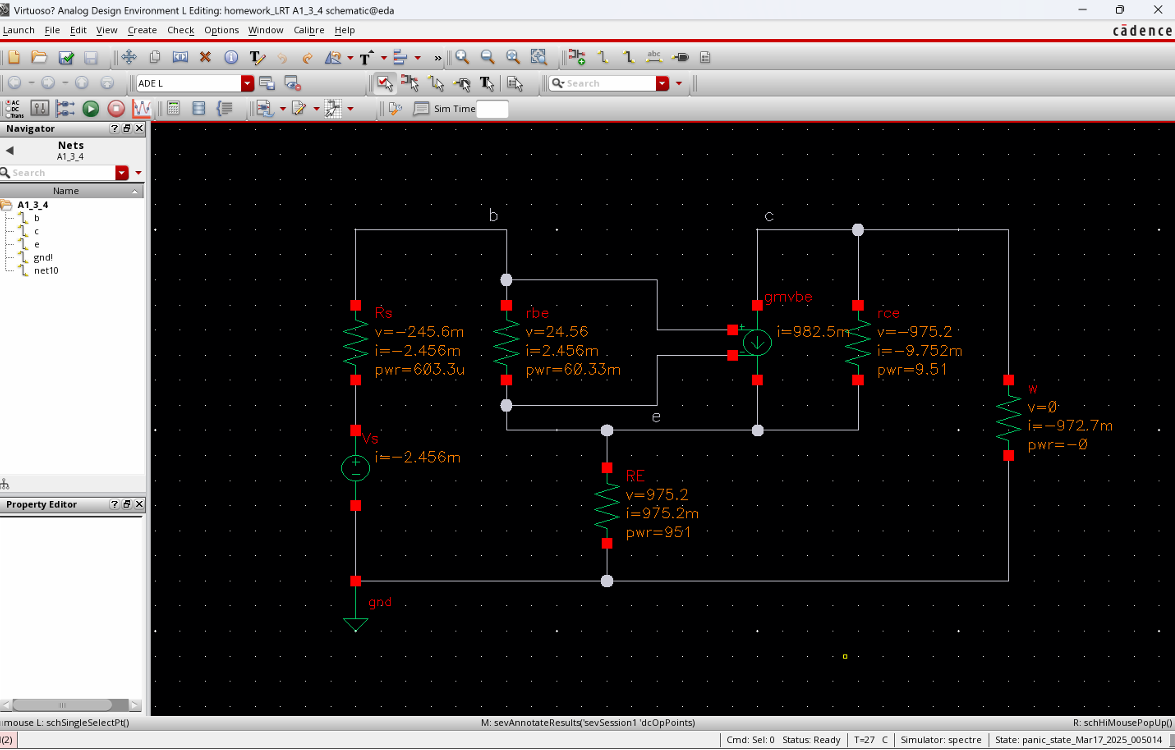
\includegraphics[width=1\textwidth]{chapters/figure/A4/A4IN.png}
\caption{等效诺顿电流源仿真结果}
\label{等效诺顿电流源仿真结果}
\end{figure}

\tt{$V_{s}=1kV$,$I_{N}=-972.7mA$，仿真得到等效诺顿电流源为$I_N=-972.7uS$，与理论计算结果一致}